\subsubsection{Ý tưởng}
Selection Sort là thuật toán sắp xếp dựa trên so sánh. Thuật toán này sắp xếp một mảng bằng cách chọn đi chọn lại phần tử nhỏ nhất (hoặc lớn nhất) từ phần chưa được sắp xếp và hoán đổi nó với phần tử chưa được sắp xếp đầu tiên. Quá trình này tiếp tục cho đến khi toàn bộ mảng được sắp xếp.
\begin{enumerate}
    \item Đầu tiên chúng ta tìm phần tử nhỏ nhất và hoán đổi nó với phần tử đầu tiên. 
    Bằng cách này, chúng ta sẽ có được phần tử nhỏ nhất ở đúng vị trí của nó.
    
    \item Sau đó, chúng ta tìm phần tử nhỏ nhất trong số các phần tử còn lại 
    (hoặc phần tử nhỏ thứ hai) và hoán đổi nó với phần tử thứ hai.
    
    \item Chúng ta tiếp tục làm như vậy cho đến khi di chuyển được tất cả các thành phần đến đúng vị trí.
\end{enumerate}
\subsubsection{Mã giả}

\begin{algorithm}[H]
    \caption{Selection Sort}
    \begin{algorithmic}[1]
    \Procedure{SelectionSort}{$arr, n$}
        \State \textbf{Input:} Mảng $arr$ gồm $n$ phần tử
        \State \textbf{Output:} Mảng $arr$ được sắp xếp
        
        \For {$i \gets 0$ \textbf{to} $n-1$}
            \State $minIdx \gets i$
            \For {$j \gets i+1$ \textbf{to} $n-1$}
                \If{$arr[j] < arr[minIdx]$}
                    \State $minIdx \gets j$
                \EndIf
            \EndFor
            \If{$minIdx \neq i$}
                \State \textbf{swap} $arr[i]$ \textbf{and} $arr[minIdx]$
            \EndIf
        \EndFor
    \EndProcedure
    \end{algorithmic}
    
\end{algorithm}
\newpage
\subsubsection{Ví dụ}
Giả sử chúng ta có mảng ban đầu: $[42, 17, 93, 58, 21, 76, 34]$. Dưới đây là các bước thực hiện Selection sort minh họa bằng hình ảnh:

\begin{figure}[H]
    \centering
    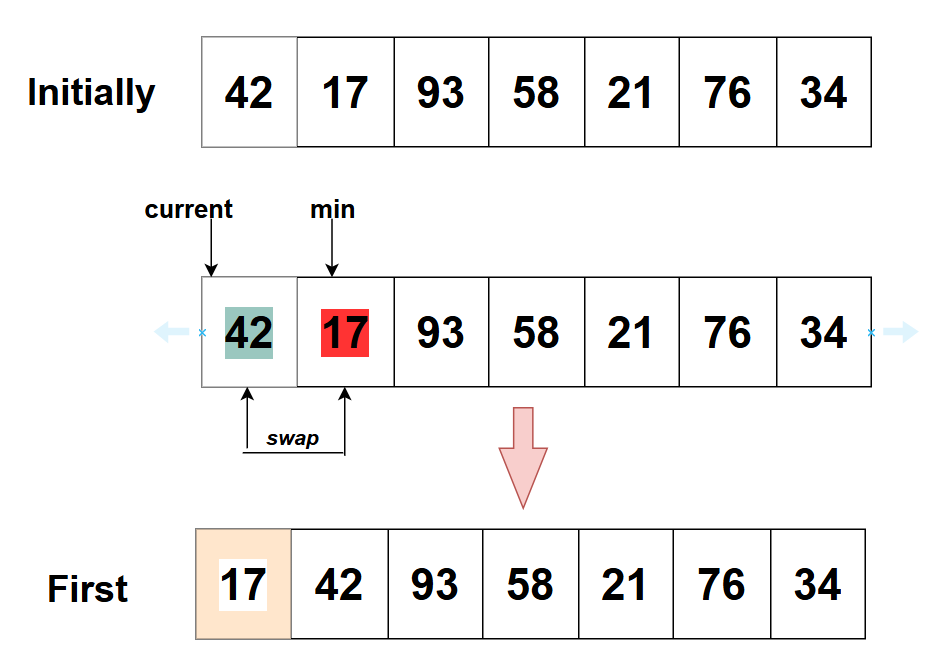
\includegraphics[width=0.7\textwidth]{img/selection sort/1.png}
    
\end{figure}

\begin{itemize}
\item Bắt đầu với phần tử đầu tiên(vị trí \textbf{curr}), chạy từ \textbf{curr} đến cuối mảng tìm phần tử nhỏ nhất (vị trí \textbf{min}) rồi hoán đổi hai phần tử ở vị trí \textbf{curr} và \textbf{min}. 
\begin{figure}[H]
    \centering
    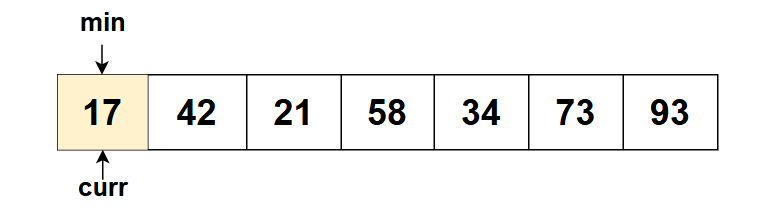
\includegraphics[width=0.7\textwidth]{img/selection sort/2.png}
    \caption{\textbf{curr} và \textbf{min} trùng nhau do 17 là phần tử nhỏ nhất}
\end{figure}

\begin{figure}[H]
    \centering
    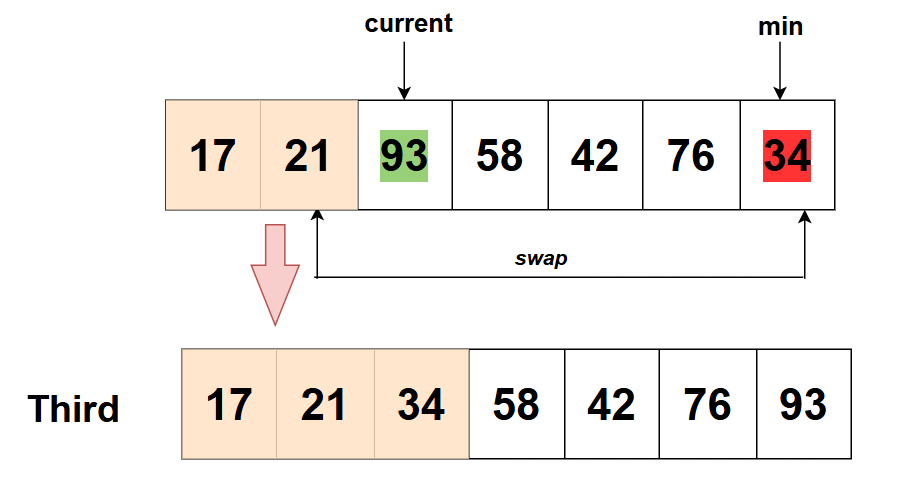
\includegraphics[width=0.7\textwidth]{img/selection sort/3.png}
    \caption{kết quả lần hoán vị đầu tiên.}
\end{figure}

\item Tiếp tục tăng \textbf{curr}, phần tử tiếp theo là vị trí \textbf{curr}, duyệt đến cuối mảng tìm phần tử nhỏ nhất (vị trí \textbf{min}) rồi hoán vị hai phần tử \textbf{curr} và \textbf{min}. Thực hiện tương tự cho đến khi mảng được sắp xếp.

\begin{figure}[H]
    \centering
    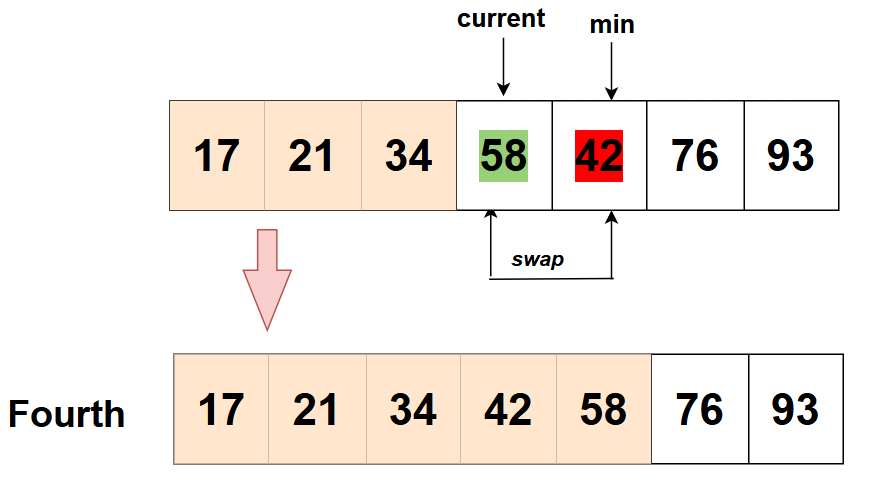
\includegraphics[width=0.7\textwidth]{img/selection sort/4.png}
    
\end{figure}

\begin{figure}[H]
    \centering
    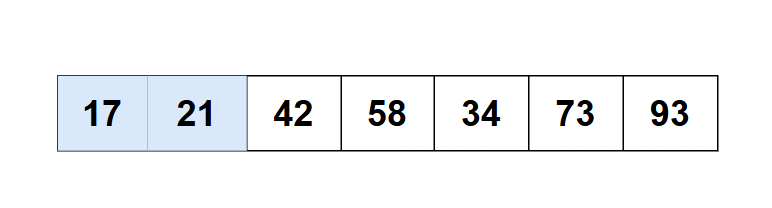
\includegraphics[width=0.7\textwidth]{img/selection sort/5.png} 
\end{figure}

\begin{figure}[H]
    \centering
    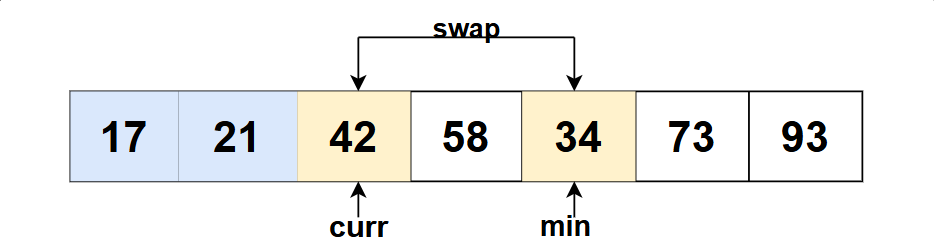
\includegraphics[width=0.7\textwidth]{img/selection sort/6.png} 
\end{figure}

\begin{figure}[H]
    \centering
    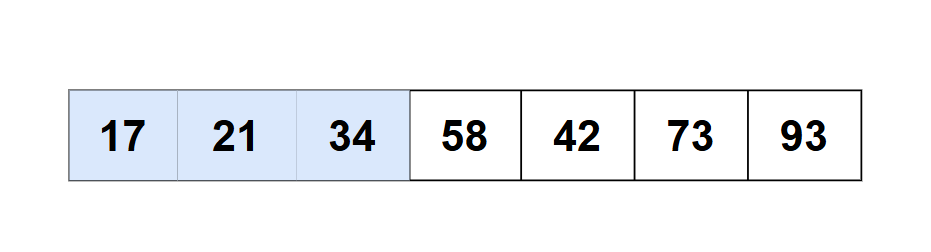
\includegraphics[width=0.7\textwidth]{img/selection sort/7.png} 
\end{figure}

\begin{figure}[H]
    \centering
    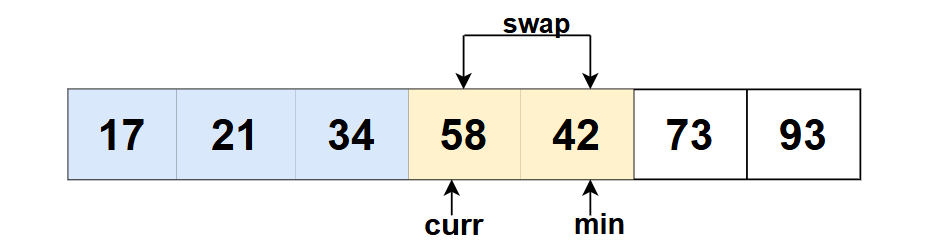
\includegraphics[width=0.7\textwidth]{img/selection sort/8.png} 
\end{figure}

\begin{figure}[H]
    \centering
    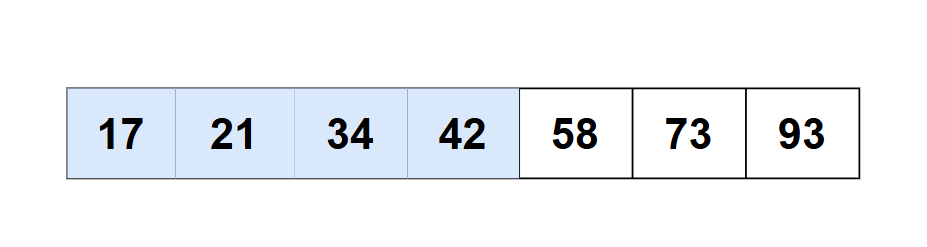
\includegraphics[width=0.7\textwidth]{img/selection sort/9.png} 
\end{figure}

\begin{figure}[H]
    \centering
    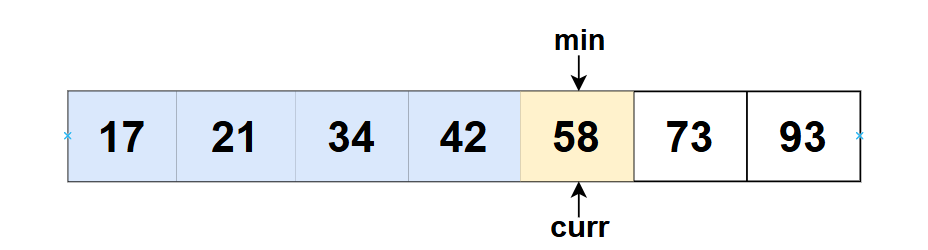
\includegraphics[width=0.7\textwidth]{img/selection sort/10.png} 
\end{figure}

\begin{figure}[H]
    \centering
    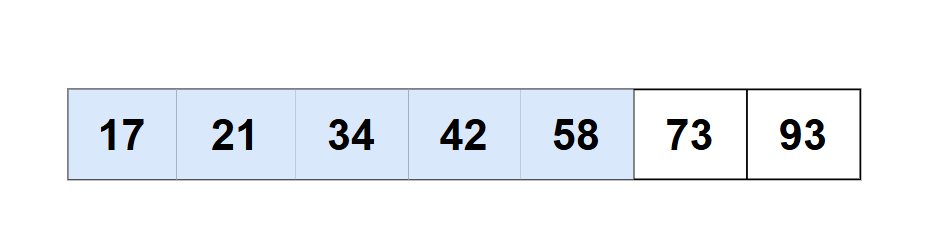
\includegraphics[width=0.7\textwidth]{img/selection sort/11.png} 
\end{figure}

\begin{figure}[H]
    \centering
    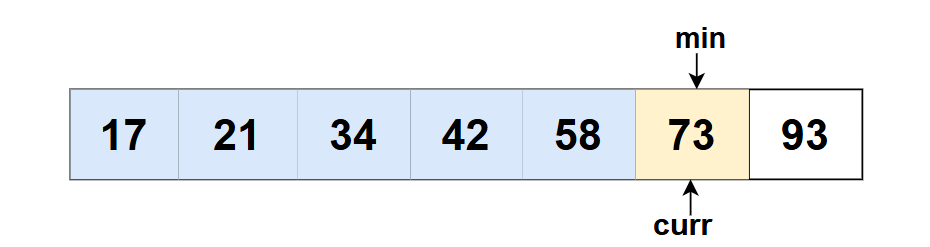
\includegraphics[width=0.7\textwidth]{img/selection sort/12.png} 
\end{figure}

\begin{figure}[H]
    \centering
    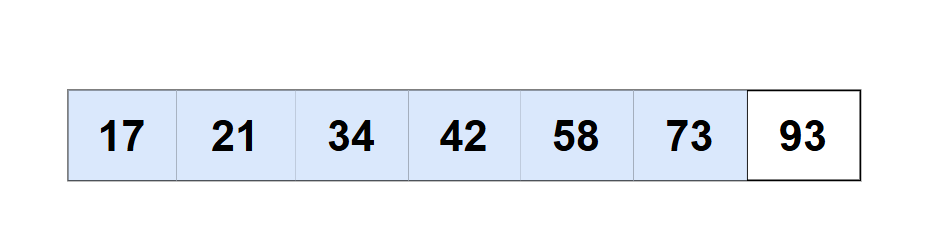
\includegraphics[width=0.7\textwidth]{img/selection sort/13.png} 
\end{figure}

\begin{figure}[H]
    \centering
    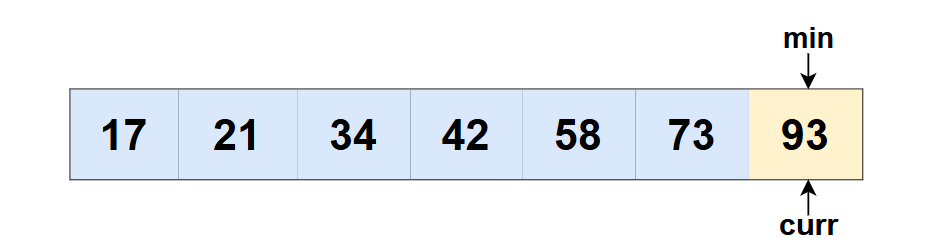
\includegraphics[width=0.7\textwidth]{img/selection sort/14.png} 
\end{figure}

\begin{figure}[H]
    \centering
    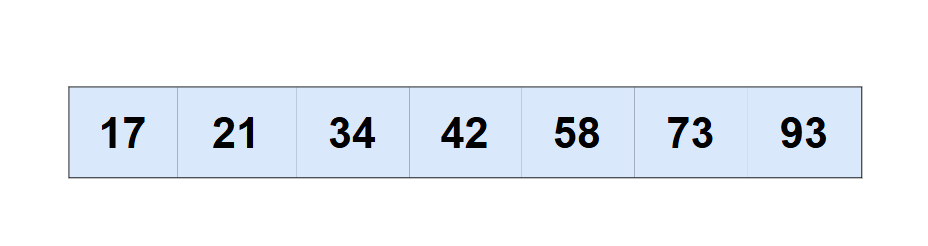
\includegraphics[width=0.7\textwidth]{img/selection sort/15.png} 
    \caption{Mảng đã được sắp xếp.}
\end{figure}


\end{itemize}

